\documentclass[tikz,border=10pt]{standalone}
\usepackage{amsmath}
\usepackage{bm}
\usetikzlibrary{calc}


\begin{document}
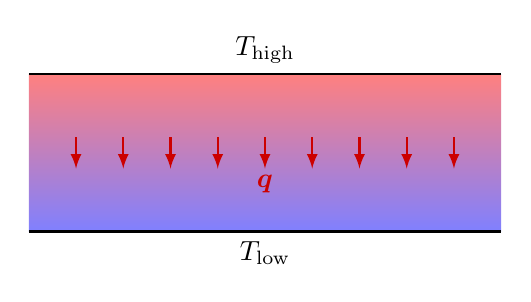
\begin{tikzpicture}
    \def\H{2.0};
    \def\L{6.0};

    \shade[top color=red!50, bottom color = blue!50] (0,0) rectangle ++(\L,\H);
    \draw[thick,black] (0,\H)--++(\L,0) node[pos=0.5, above,anchor = south] {$T_\text{high}$};
    \draw[thick,black] (0,0)--++(\L,0) node[pos=0.5, below, anchor=north] {$T_\text{low}$};

    \foreach \y in {0.1, 0.2, ..., 0.9} {
      \draw[-latex,thick,color=red!80!black] (\y*\L,0.6*\H)--++(0,-0.2*\H);
    }

    \node[color=red!80!black] at (0.5*\L,0.3*\H) {$\bm{q}$};
    
\end{tikzpicture}
\end{document}
